\documentclass[11pt,]{article}
\usepackage{lmodern}

\usepackage{amssymb,amsmath}
\usepackage{ifxetex,ifluatex}
\usepackage{fixltx2e} % provides \textsubscript
\ifnum 0\ifxetex 1\fi\ifluatex 1\fi=0 % if pdftex
  \usepackage[T1]{fontenc}
  \usepackage[utf8]{inputenc}
\else % if luatex or xelatex
  \ifxetex
    \usepackage{mathspec}
    \usepackage{xltxtra,xunicode}
  \else
    \usepackage{fontspec}
  \fi
  \defaultfontfeatures{Mapping=tex-text,Scale=MatchLowercase}
  \newcommand{\euro}{€}
\fi
% use upquote if available, for straight quotes in verbatim environments
\IfFileExists{upquote.sty}{\usepackage{upquote}}{}
% use microtype if available
\IfFileExists{microtype.sty}{%
\usepackage{microtype}
\UseMicrotypeSet[protrusion]{basicmath} % disable protrusion for tt fonts
}{}
\usepackage[lmargin=5cm,rmargin=2.5cm,tmargin=2.5cm,bmargin=2.5cm]{geometry}

%% citation setup

\usepackage{csquotes}

\usepackage[backend=biber, maxbibnames = 99, style = apa]{biblatex}
\setlength\bibitemsep{1.5\itemsep}
\bibliography{references.bib}
\usepackage{longtable,booktabs}
\usepackage{graphicx}
\makeatletter
\def\maxwidth{\ifdim\Gin@nat@width>\linewidth\linewidth\else\Gin@nat@width\fi}
\def\maxheight{\ifdim\Gin@nat@height>\textheight\textheight\else\Gin@nat@height\fi}
\makeatother
% Scale images if necessary, so that they will not overflow the page
% margins by default, and it is still possible to overwrite the defaults
% using explicit options in \includegraphics[width, height, ...]{}
\setkeys{Gin}{width=\maxwidth,height=\maxheight,keepaspectratio}
\ifxetex
  \usepackage[setpagesize=false, % page size defined by xetex
              unicode=false, % unicode breaks when used with xetex
              xetex]{hyperref}
\else
  \usepackage[unicode=true]{hyperref}
\fi
\hypersetup{breaklinks=true,
            bookmarks=true,
            pdfauthor={Jonathan Berrisch, Timo Rammert},
            pdftitle={A Forecasting Study on Global Wine Sales},
            colorlinks=true,
            citecolor=blue,
            urlcolor=blue,
            linkcolor=magenta,
            pdfborder={0 0 0}}
\urlstyle{same}  % don't use monospace font for urls
\setlength{\parindent}{0pt}
\setlength{\parskip}{6pt plus 2pt minus 1pt}
\setlength{\emergencystretch}{3em}  % prevent overfull lines
\setcounter{secnumdepth}{5}

%%% Use protect on footnotes to avoid problems with footnotes in titles
\let\rmarkdownfootnote\footnote%
\def\footnote{\protect\rmarkdownfootnote}

%%% Change title format to be more compact
\usepackage{titling}

% Create subtitle command for use in maketitle
\newcommand{\subtitle}[1]{
  \posttitle{
    \begin{center}\large#1\end{center}
    }
}

\setlength{\droptitle}{-2em}
  \title{A Forecasting Study on Global Wine Sales}
  \pretitle{\vspace{\droptitle}\centering\huge}
  \posttitle{\par}
\subtitle{Statistical Learning}
  \author{Jonathan Berrisch, Timo Rammert}
  \preauthor{\centering\large\emph}
  \postauthor{\par}
  \predate{\centering\large\emph}
  \postdate{\par}
  \date{today}


%% linespread settings

\usepackage{setspace}

\onehalfspacing

% Language Setup

\usepackage{ifthen}
\usepackage{iflang}
\usepackage[super]{nth}
\usepackage[ngerman, english]{babel}

\begin{document}

\selectlanguage{english}


%\maketitle

\begin{titlepage}
  \noindent\begin{minipage}{0.6\textwidth}
	  \IfLanguageName{english}{University of Duisburg-Essen}{Universität Duisburg-Essen}\\
	  \IfLanguageName{english}{Faculty of Business Administration and Economics}{Fakultät für Wirtschaftswissensschaften}\\
	  \IfLanguageName{english}{Chair of Econometrics}{Lehrstuhl für Ökonometrie}\\
  \end{minipage}
	\begin{minipage}{0.4\textwidth}
	  \begin{flushright}
  	  \vspace{-0.5cm}
      \IfLanguageName{english}{\includegraphics*[width=5cm]{Includes/duelogo_en.png}}{\includegraphics*[width=5cm]{Includes/duelogo_de.png}}
	  \end{flushright}
	\end{minipage}
  \\
  \vspace{1.5cm}
  \begin{center}
  \huge{A Forecasting Study on Global Wine Sales}\\
  \vspace{.25cm}
  \Large{Statistical Learning}\\
  \vspace{0.5cm}
  \large{Term Paper}\\
  \vspace{1cm}
  \large{
  \IfLanguageName{english}{Submitted to the Faculty of \\ Business Administration and Economics \\at the \\University of Duisburg-Essen}{Vorgelegt der \\Fakultät für Wirtschaftswissenschaften der \\ Universität Duisburg-Essen}\\}
  \vspace{0.75cm}
  \large{\IfLanguageName{english}{from:}{von:}}\\
  \vspace{0.5cm}
  Jonathan Berrisch, Timo Rammert\\
  \end{center}
  \vspace{4cm}

  \noindent\begin{minipage}[t]{0.3\textwidth}
  \IfLanguageName{english}{Matriculation Number}{Matrikelnummer}
  \end{minipage}
  \begin{minipage}[t]{0.7\textwidth}
  \hspace{1cm}3071485 \textbar{} XXXXXXX
  \end{minipage}

  \noindent\begin{minipage}[t]{0.3\textwidth}
  \IfLanguageName{english}{Study Path:}{Studienfach:}
  \end{minipage}
  \begin{minipage}[t]{0.7\textwidth}
  \hspace{1cm}Study Path
  \end{minipage}

  \noindent\begin{minipage}[t]{0.3\textwidth}
  \IfLanguageName{english}{Reviewer:}{Erstgutachter:}
  \end{minipage}
  \begin{minipage}[t]{0.7\textwidth}
  \hspace{1cm}Prof.~Dr.~Christoph Hanck
  \end{minipage}

  \noindent\begin{minipage}[t]{0.3\textwidth}
  \IfLanguageName{english}{Secondary Reviewer:}{Zweitgutachter}
  \end{minipage}
  \begin{minipage}[t]{0.7\textwidth}
  \hspace{1cm}NA
  \end{minipage}

  \noindent\begin{minipage}[t]{0.3\textwidth}
  Semester:
  \end{minipage}
  \begin{minipage}[t]{0.7\textwidth}
  \hspace{1cm}\IfLanguageName{english}{\nth{1} Semester}{1. Fachsemester}
  \end{minipage}

  \noindent\begin{minipage}[t]{0.3\textwidth}
  \IfLanguageName{english}{Graduation (est.):}{Vsl. Studienabschluss:}
  \end{minipage}
  \begin{minipage}[t]{0.7\textwidth}
  \hspace{1cm}Summer Term 2019
  \end{minipage}

  \noindent\begin{minipage}[t]{0.3\textwidth}
  \IfLanguageName{english}{Deadline:}{Abgabefrist:}
  \end{minipage}
  \begin{minipage}[t]{0.7\textwidth}
  \hspace{1cm}Aug.~27th 2019
  \end{minipage}

\end{titlepage}


\pagenumbering{Roman} 
{
\hypersetup{linkcolor=black}
\setcounter{tocdepth}{3}
\tableofcontents
}
\newpage
\listoftables
\newpage
\listoffigures
\newpage
\pagenumbering{arabic} 
\hypertarget{introduction}{%
\section{Introduction}\label{introduction}}

This paper presents a forecasting study on global wine sales. This study
is based on the friberg gronqvist wine data set which is publicly
available and was previously analyzed by {[}Textcite AER Friberg,
Grönqvist{]}. Recent technological advancements led to an significant
increase in techniques that are computationally demanding and are
potentially outperforming classical statistical methods, especially in
terms of forecasting. Those techniques are usually reffered as
statistical- or machine learning methods.

We presents various models which are increasingly complex. Those models
potentially gain forecasting power while losing interpretability. The
applied models range from linear regressions to tree based methods like
Random Forests and Boosting. The goal is to develop the best possible
model to forecast wine sales in litre.

The remainder of this paper is strctures as followes. Chapter 2 gives
and overview about the dataset and the preprocessing. Chapter 3
describes the validation approach. Chapter 4 presents the models and
their specification. Chapter 5 provides the results, a conclusion and
some ideas for future research.

\hypertarget{data-and-variables}{%
\section{Data and Variables}\label{data-and-variables}}

The datset contains 145179 observations with 59 variables. The variables
include the name of the wine, the country of origin, its price, the
amount sold per week in litre, the taste segment and variables releated
to diffeerent reviews among others. We need to omit two variables
beforehand, namely \enquote{time\_segm\_price} and \enquote{artikpr},
because those are combinations of other existing variables. Hence
inclusion would lead to the problem of multicollinearity in some models.
After omitting those two we have left the following types of variables:

\begin{longtable}[]{@{}rrrr@{}}
\toprule
Date & factor & logical & numeric\tabularnewline
\midrule
\endhead
1 & 8 & 19 & 29\tabularnewline
\bottomrule
\end{longtable}

Figure 1 depicts the amount of missing values in each variable. The
number of complete cases would be zero without further selection.
Therefore we exclude every variable with a ratio of missing values that
exceeds \(50\%\). In consequence 41416 Observations with 45 Variables
are used for building the forecasting models.

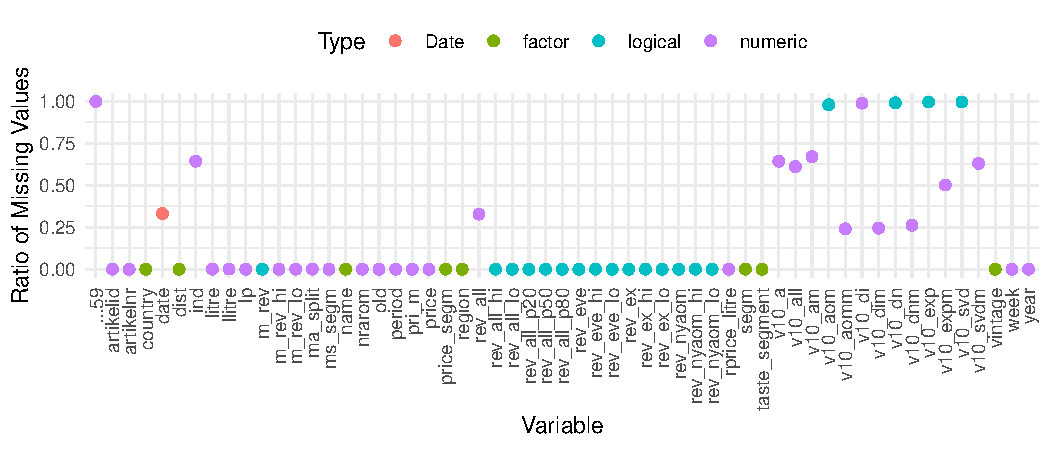
\includegraphics{../00_data/output_paper/02_missings.pdf}

\hypertarget{validation-approach}{%
\section{Validation Approach}\label{validation-approach}}

Here we go describing our approach to evaluate overall model performance
and tune parameters. =\textgreater{} CV and loops for
hyperparameters\ldots{} We should make it very clear that every rmse
that is presented is the results of a 5 fold cross validation!

\hypertarget{analysis}{%
\section{Analysis}\label{analysis}}

\hypertarget{mean-regression-and-linear-regression}{%
\subsection{Mean Regression and Linear
Regression}\label{mean-regression-and-linear-regression}}

At first a mean regression and a linear regression are calculated and
used as a baseline for further methods. For comparison of the different
models, the Root Mean Sqaured Error (RMSE)
\[\sqrt{\frac{1}{n}\sum_{i = 1}^{n}\left(y_i-\hat{y}_i\right)^2}\] is
calculated.

\begin{figure}
\centering
\includegraphics{term_paper_files/figure-latex/Mean Regression-1.pdf}
\caption{Residuals of the Mean Regression.}
\end{figure}

\begin{verbatim}
##        mod    rmse
## 1     Mean 2193578
## 2 Basic_lm      NA
\end{verbatim}

\begin{figure}
\centering
\includegraphics{term_paper_files/figure-latex/ResPlotMR-1.pdf}
\caption{Histogram and Density of the Residuals of the Mean Regression.}
\end{figure}

\hypertarget{subset-selection}{%
\subsection{Subset Selection}\label{subset-selection}}

\hypertarget{forward-stepwise-selection}{%
\subsubsection{Forward Stepwise
Selection}\label{forward-stepwise-selection}}

\hypertarget{backward-stepwise-selection}{%
\subsubsection{Backward Stepwise
Selection}\label{backward-stepwise-selection}}

\hypertarget{lasso}{%
\subsection{Lasso}\label{lasso}}

\hypertarget{pls-and-pcr}{%
\subsection{PLS and PCR}\label{pls-and-pcr}}

\hypertarget{splines}{%
\subsection{Splines}\label{splines}}

\hypertarget{regression-trees-and-random-forests}{%
\subsection{Regression Trees and Random
Forests}\label{regression-trees-and-random-forests}}

\hypertarget{regression-tree}{%
\subsubsection{Regression Tree}\label{regression-tree}}

\hypertarget{pruned-tree}{%
\subsubsection{Pruned Tree}\label{pruned-tree}}

\hypertarget{bagging}{%
\subsubsection{Bagging}\label{bagging}}

\hypertarget{random-forest}{%
\subsubsection{Random Forest}\label{random-forest}}

\hypertarget{boosting}{%
\subsubsection{Boosting}\label{boosting}}

\hypertarget{conclusion}{%
\section{Conclusion}\label{conclusion}}

\pagebreak

\hypertarget{citations}{%
\subsection{Citations}\label{citations}}

\pagebreak

\hypertarget{annotations}{%
\subsection{Annotations}\label{annotations}}

\hypertarget{overview-over-the-rmses}{%
\subsubsection{Overview over the RMSEs}\label{overview-over-the-rmses}}

\begin{tabular}{l|r|r}
\hline
Method & RMSE & No..of.Variables\\
\hline
Mean-Regression & 0 & 0\\
\hline
Linear Regression & 0 & 0\\
\hline
Forword Stepwise Selection & 0 & 0\\
\hline
Backward Stepwise Selection & 0 & 0\\
\hline
Regression Tree & 0 & 0\\
\hline
Pruned Tree & 0 & 0\\
\hline
Random Forest & 0 & 0\\
\hline
\end{tabular}
\renewcommand*{\mkbibnamefamily}[1]{\textbf{#1}}
\renewcommand*{\mkbibnamegiven}[1]{\textbf{#1}}
\renewcommand*{\mkbibnameprefix}[1]{\textbf{#1}}
\renewcommand*{\mkbibnamesuffix}[1]{\textbf{#1}}
\printbibliography[title=References]

\newpage
\textbf{Eidesstattliche Versicherung}

\bigskip

Ich versichere an Eides statt durch meine Unterschrift, dass ich die vorstehende Arbeit selbständig und ohne fremde Hilfe angefertigt und alle Stellen, die ich wörtlich oder annähernd wörtlich aus Veröffentlichungen entnommen habe, als solche kenntlich gemacht habe, mich auch keiner anderen als der angegebenen Literatur oder sonstiger Hilfsmittel bedient habe. Die Arbeit hat in dieser oder ähnlicher Form noch keiner anderen Prüfungsbehörde vorgelegen.

\vspace{1cm}
\rule{0pt}{2\baselineskip} %
\par\noindent\makebox[2.25in]{\indent Essen, den \hrulefill} \hfill\makebox[2.25in]{\hrulefill}%
\par\noindent\makebox[2.25in][l]{} \hfill\makebox[2.25in][c]{Jonathan Berrisch, Timo Rammert}%


\end{document}
